\documentclass[11pt,a4paper]{article}
\usepackage[utf8]{inputenc}
\usepackage[english]{babel}
\usepackage{amsmath}
\usepackage{amsfonts}
\usepackage{amssymb}
\usepackage{mathrsfs}
\usepackage{gensymb}
\usepackage{fancyhdr}
\usepackage[left=1.5cm,right=1.5cm,top=2.5cm,bottom=2cm]{geometry}
\usepackage{adjustbox}
\usepackage{booktabs}  
\usepackage{threeparttable} 
\usepackage{makecell}
\usepackage{parskip}
\usepackage{graphicx}
\usepackage{listings}

\begin{document}
\title{Final Project}

\pagestyle{fancy}

{
\fancyhf{}
\rhead{30 November 2017}
\lhead{Yunzhe (Jack) Li \& Xiaofei Li} 
\cfoot{\thepage}
}

\begin{center}
\subsection*{137 Time Series Final Project\\The Research on Popularity of League of Legends \\Yunzhe Li 914361644\\Xiaofei Li 914516062 }
\end{center}

\section*{Abstract}
We are interested in the popularity of the on-line video game League of Legends (LOL) and collect 96 monthly data from Google Trend through November 2009 to October 2017 to analyze and predict them applying Time Series. Firstly, we use the fifth degree polynomial model to estimate the trend part and remove them successfully. Meanwhile, we also consider specific activities that affected the trend most and make improved model to fit it better. Secondly, we estimate the seasonality part by small trend method and remove them to get a stationary random part by checking its ACF, PACF and so on. While by comparing the random part  with de-trending part, we get the conclusion that the seasonality has little affect on them. After that, we fit AR(1) model to the random part and add the model totally to make prediction successfully. Moreover, we make spectral analysis on the data and get accurate prediction. Finally, we analyze the popularity by our findings to make future forecast and provide advice to the players and on-line video game industries.


\section*{Introduction}
League of Legends (LOL) is one of the most popular on-line multi-player battle arena video game around the world. A number of young people like us are all its super fans. Therefore, we are naturally curious about how many people have interests on LOL and have the same hobby like us. On the other hand, LOL also gains much more benefits for the producers and players in competitive game area. From November 11 in 2009, the time when LOL initial released, until today, it attracts extremely large attention no matter just for fun or for industry business. Its development path is also a successful reference and providing many ideas for us. 

Taking all these factors into consideration, analysis of the popularity of LOL becomes necessary and interesting. So in our project, we will display the process of researching the popularity of LOL changing over time by using time series method we learned. On base of them, we also try to find a good pattern which we hopefully can be a successful reference or providing useful ideas for its fans and industry business.

\subsection*{Data Description}
Our data is the popularity of a multilayer on-line battle arena video game, League of Legends. We collect our data from Google Trend, and the website is https://trends.google.com/trends/.
We have monthly data of the popularity of LOL through November 2009 to October 2017, where the sample size is 96. The data from Google Trend has range 0 to 100, where the the highest point will be considered as 100, and other points are the proportion of that peak number. This dataset includes the initial released LOL data until recently October this year. For evaluating our model, we decide to hide one year data, from 11/2016 to 10/2017.

\newpage
\begin{itemize}\item
\textit{Original data plot}
\end{itemize}
\begin{center}
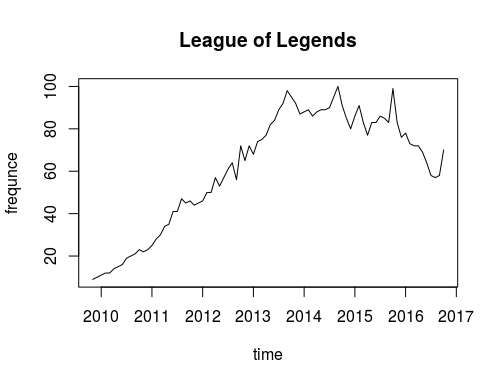
\includegraphics[width=0.5\textwidth]{Originalplot.png}

{Figure 1-1: The popularity of LOL data plot}
\end{center}

The horizontal axis is the time from 11/2009 to 10/2016. An the vertical axis is the searching frequency that stand for the popularity through 0-100. And the most interesting features of the data is that its trends has peaks or fluctuations which are affected by annual world championship. These can give us more interesting information.
\begin{itemize}\item
\textit{Data Summary statistics}
\end{itemize}
\vspace{10 mm}
\begin{center}
\begin{table}[htbp]
\begin{center}
\begin{tabular}{l  c  c  c  c  c  c  c }\hline\hline
\multicolumn{1}{c}{Variables} &     Min. &          1st Qu.&         Median&         Mean&  3rd Qu.&Max.\\ \hline
Popularity of LOL&9.0&41.0&59.5&59.6&83.0&100.0\\
\hline \hline
 \end{tabular}
 
 {Table 1-1: Summary statistics of data}
 \end{center}
\end{table}

\end{center}

\section*{Data Analysis}

On base the description of our data and analyzing the original data plot, we can find that the popularity of LOL is changing over time. And we plan to use the time series method to analyze it, which can be decomposed as trend (m$_t$) plus seasonality (s$_t$) plus random part (X$_t$). Such as:

\begin{center}
X$_t$ = m$_t$ + s$_t$ + Y$_t$
\end{center} 

After we estimating and removing the trend part and seasonality part, we try to pick a model fitted the random part.

\subparagraph{a)Exploratory Analysis}\mbox{}\\ 
\begin{itemize}\item

\textit{Estimated Trend part and Remove them}

For the trend part, we fit the polynomial model by "lm" function in R to the data performed. We get the AIC and BIC value when we fit polynomial model from the first degree to the sixth degree like the table below.
{
\begin{table}[htbp]
\centering
\begin{tabular}{l  c  c  c  c  c  c  c }\hline\hline
\multicolumn{1}{c}{The degree of Polynomial} & 1& 2&3& 4&5&6\\ \hline
AIC&711.6328 &583.3724& 517.8389 &511.4006 &510.1923 &511.5385\\
BIC&718.9253& 593.0957&529.9930 &525.9855& 527.2080 &530.9851\\
\hline \hline
 \end{tabular}
\end{table}
}
 \begin{center}
 {Table 2-1: AIC and BIC value of different degrees of polynomial}
 \end{center}
 

By comparing the value of AIC and BIC, we find that the fifth degree has both the smallest AIC and BIC, so we choose the fifth degree model to fit the trend. The result shows below.

\begin{center}
\includegraphics[width=0.5\textwidth]{5-degree_trend_.png}

{Figure 2-1: Power 5 Polynomial Fitting Model}
\end{center}

By looking at the plot, we find that there is no obvious seasonality component. And it is like what we think (We will show it in Appendix). But there are some recognizable spikes in the plot. After some researches, we find that those might be caused by world championship. Schedule of World championships is following: Season1-6/2011, Season2-10/2012, Season3: 9-10/2013 S4: 9/2013-10/2014, Season5-10/2015,  Season6-10/2016, Season7-10/2017.\newline

There is no significant spike for Season  1, therefore we choose to only use Season 2 to Season 6 for building our model.
We add an indicator column in our design matrix, 1 means there is a world championship and 0 mean there is not. The AIC and BIC of new model are 465.9622 and 485.4088 respectively, which are significantly smaller than the AIC and BIC for previous model. It looks like following:	

\begin{center}
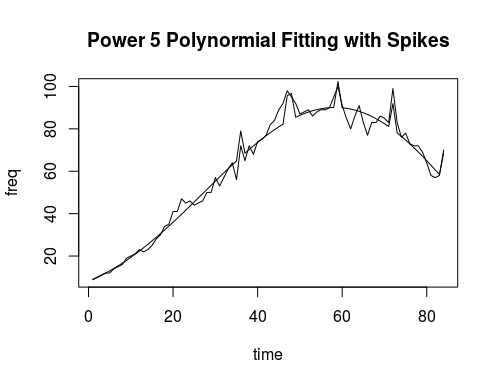
\includegraphics[width=0.5\textwidth]{WithSpikes.png}

{Figure 2-2: Power 5 Improved Polynomial Fitting Model with Spikes}
\end{center}
Finally, to de-trend, we use the original data subtract the fitted values from improved model. The plot is in Figure 2-3:


\includegraphics[width=0.5\textwidth]{after_detrend.png}
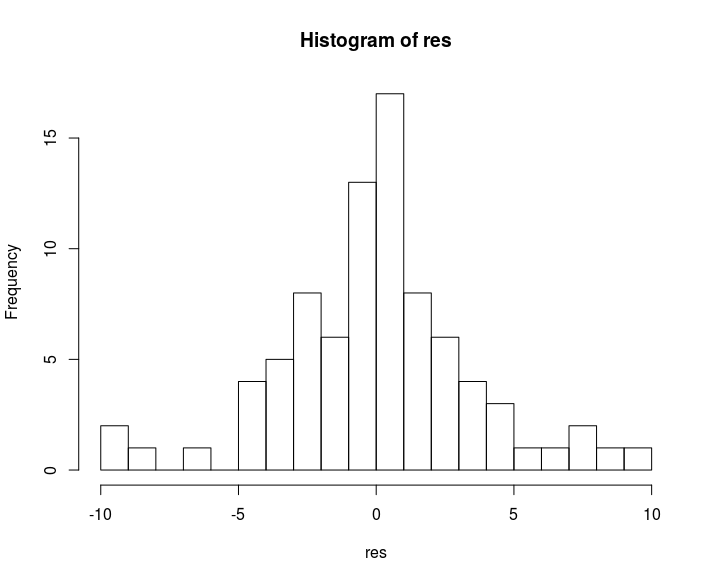
\includegraphics[width=0.5\textwidth]{Hist_res.png}
\hspace{3cm}{Figure 2-3: De-trending Data Plot}\hspace{4cm} {Figure 2-4: Histogram of De-trending Data}

By looking at Figure2-3, we could assume the data after de-trending is stationary. And from the Figure2-4 above, we can tell that the residuals are normally distributed without dependence.




\subparagraph{b)Model Selection}\mbox{}\\
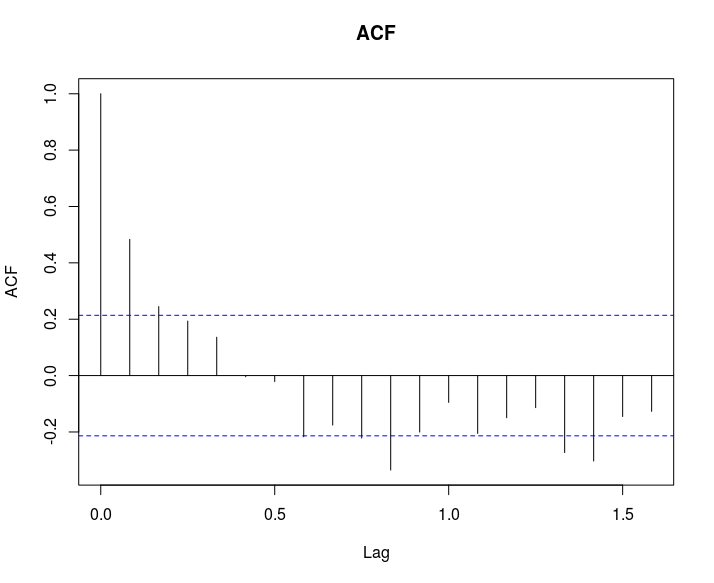
\includegraphics[width=0.5\textwidth]{ACF.png}
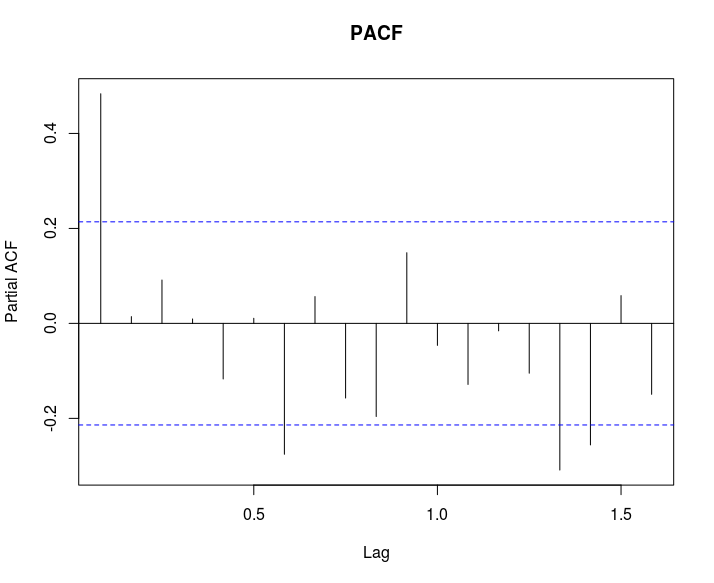
\includegraphics[width=0.5\textwidth]{PACF.png}
\hspace{3cm}{Figure 2-5: ACF of De-trending Data Plot}\hspace{2cm} {Figure 2-6: PACF of De-trending Data Plot}

In Figure 2-5, Figure2-6  above, the unit of lags are year, so spikes mean monthly lag. 
By analyzing the ACF and PACF figures, we can find that it looks like ARMA(1,1) model, but by using the function auto.arima(), we get the AR(1) model with $\varphi_1$ = 0.4789, which has the smallest prediction error. Then the AR(1) estimation is like Figure 2-7:

\end{itemize}


\begin{center}
\includegraphics[width=0.5\textwidth]{auto_arma.png}
\end{center}
\begin{center}
{Figure 2-7: AR(1) Estimation of Stationary Series}
\end{center}
And we find that it looks approximatively similar of the original  data. So we choose AR(1) model to fit our random part.
\subparagraph{c) Prediction}\mbox{}\\ 

So when we get our random part model in part (b), we add smooth trend from part (a) to get the total model to fit the original data. We use "forecast()" function in R to make prediction like Figure 2-8, and our constructed confidence interval is 95 percentiles. 
The two red lines are the upper band and lower band of our prediction respectively, and the blue one is the mean of the estimation. Compared to the original data in the curve like dark red line, we can find the prediction is almost same.

\begin{center}
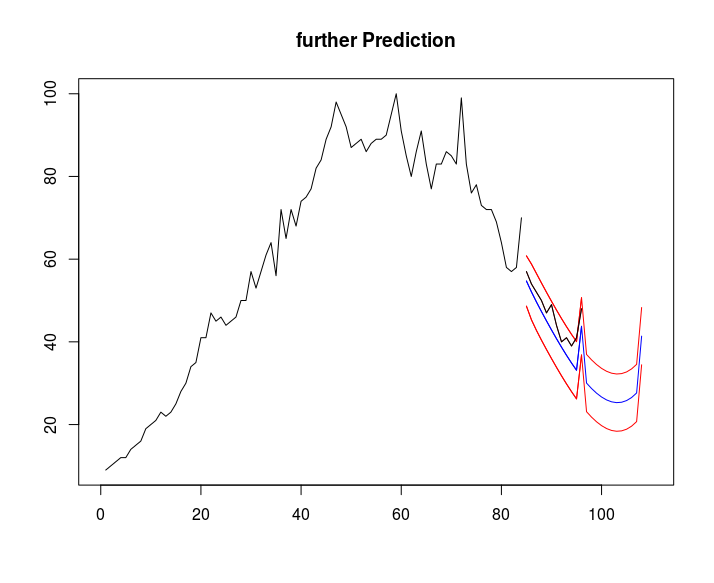
\includegraphics[width=0.5\textwidth]{furPre.png}
\end{center}
\begin{center}
{Figure 2-8: Prediction of the Popularity of LOL}
\end{center}
\newpage
\section*{Extra Credit: Spectral Analysis}
\subparagraph{a) Picking a Model}\mbox{}\\ 
\begin{center}
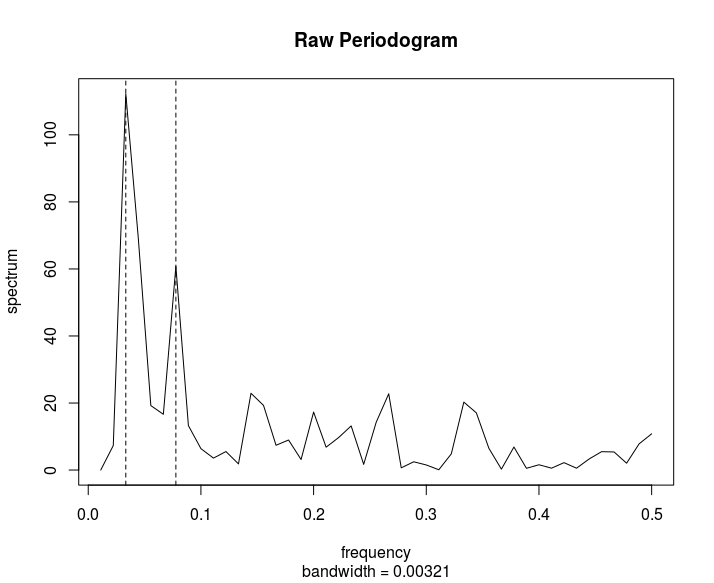
\includegraphics[width=0.5\textwidth]{Periodogram.png}
\end{center}
\begin{center}
{Figure 3-1: Periodogram of  Data Plot}
\end{center}

We make our Periodogram by using the function "spec.pgram()" like Figure  . And get the two peak at specific frequency. The two frequency is  0.0333 and 0.0778 respectively. And the total area under the two peaks is about 0.4952545 by calculation. And the data collected between the two peak can explain about 50 percents variance in the random part.
The graph below shows the estimation of the stationary series.
\begin{center}
\includegraphics[width=0.5\textwidth]{estimate.png}
\end{center}
\begin{center}
{Figure 3-2: Estimation of Data Plot}
\end{center}

\subparagraph{b) Prediction}\mbox{}\\ 
And we use the spectral analysis to do the prediction like these two figures.
The red lines our prediction. It fits the model very well but a little bit under estimate.
\begin{center}
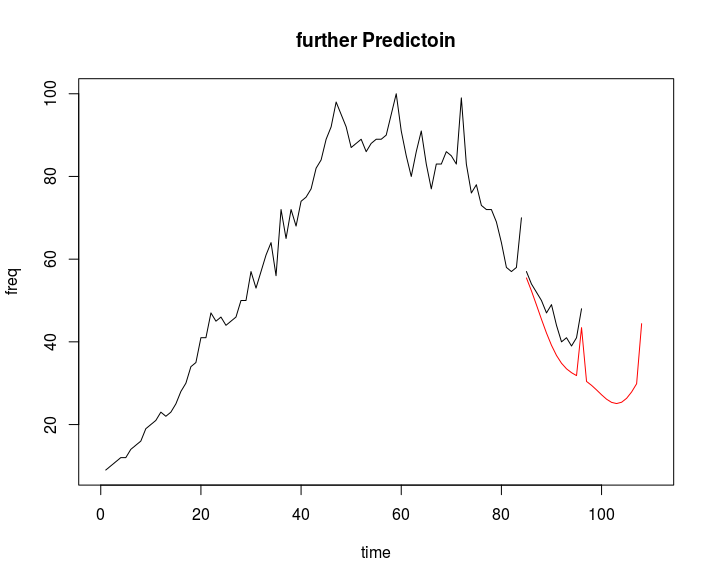
\includegraphics[width=0.5\textwidth]{furPrePer.png}
\end{center}
\begin{center}
{Figure 3-4: Estimation of Data Plot}
\end{center}
\section*{Discussion}
We use the fifth degree polynomial model with an extra indicator term, which stands for the world championship month, to fit the trend part. After de-seasonality, we realize there is no obvious seasonal component in our data, that means the seasonality has little affect in our model, therefore we choose to not consider the seasonal part to keep our model simpler. After de-trend, we obtain a stationary series. We use AR(1) model fit this stationary series. By adding the prediction from smooth part (trend) and random part (stationary series) together to make final prediction. And compare the prediction to the hidden data. We can conclude that it looks like the right prediction of the original data.


\section*{Conclusion}
During our project, we make accurate analysis on the popularity of LOL and predict the data successfully. These results show that when the LOL initial released, there is no many attention on them. While with the development of LOL, more and more people became interested on them. The popularity of LOL increased fast during 2011 to 2013. From October 2013 to October 2015, LOL enters high speed development time though it has some fluctuations affected by the actives and environment. After October 2015, the popularity of LOL became decreased slowly, this may because more and more competitors going into on-line video game industry. Our prediction results shows that the decreasing time will last for about two to three years though there will be little  fluctuations during the process. It can remind the industries that they can put more advertisements and tricks to attract more players in case of lasting decreasing to make loss.

On the other hand, we find that every time when it arrived the most popularity points that is according to several peaks in plots in a time quantum, there was exactly annual world championship organizing. Our analysis points that the world championship attracts much more attention and gain the most popularity time among these years. So for industries, it is a great chance for them to advertise and show the interests of LOL to players.

After that, between 2018 and 2019,  it will welcome the second increased popularity time by the improvement of technologies and money plus on expanding the market. And the players will be attracted more by the new styles on LOL and the industries will gain more from that. 

\newpage
\section*{Appendix}\begin{itemize}
\item\textit{Estimated Seasonality part and Remove them}

We use small trend method to estimate seasonality. We calculate the mean of each years' data and naturally make it as our estimator to get the seasonality as Figure 4-1. So the trend part and seasonality part of the data is like Figure 4-2.

\includegraphics[width=0.5\textwidth]{season.png}
\includegraphics[width=0.5\textwidth]{adding_season.png}   {Figure 4-1: Seasonality of  Data Plot}\hspace{2cm} {Figure 4-2: Trend part and Seasonality of Data Plot}    


\item
{R Code}
\begin{lstlisting}[language=R]
# Description:
# Analysis of online game - League of Legends searched on Google
# Data provider: Google Trend
num = as.numeric(data[,1])[1:84]
num_pred = as.numeric(data[,1])[85:96]
dat = data[,2][1:84]
dat_pred = data[,2][85:96]
lol_t = ts(num, start = c(2009,11), freq = 12)
plot(lol_t, main = "League of Legends", xlab = "time", ylab = "frequnce")

# method 1
# polynomial fitting

# checking different models
t = 1:length(num)
models = lapply(1:6, function(x) lm(lol_t~poly(t, degree = x)))
sapply(models, AIC)
sapply(models, BIC)

# choose power 5
fitmodel = lm(lol_t~poly(t, degree = 5))
plot(t, lol_t, type= "l", xlab = "time", ylab = "popularity", main = "original plot with power 5 polynormial fitting line")
lines(fitmodel$fitted.values)

# try to de-seaonality
de_trend1 = lol_t-fitmodel$fitted.values
plot(de_trend1, type = 'l', main = "After Detrend")
de_trend_matrix1 = matrix(c(rep(NA,10),de_trend1,rep(NA,2)), ncol = 12, byrow = TRUE)
trend_mean1 = apply(t(de_trend_matrix1),1,function(x) mean(x, na.rm = TRUE))
seasonality_matrix1 = rep(trend_mean1, nrow(de_trend_matrix1)-1)
plot(t, seasonality_matrix1, type = "l", main = "Seasonality")
de_seasonality1 = de_trend1 - seasonality_matrix1

plot(t, lol_t, type= "l", xlab = "", ylab = "", main = "Treand With Seasonality")
lines(seasonality_matrix1 + fitmodel$fitted.values, col = "red")

# checking residules
plot(t, de_seasonality1, type = "l") # the left part looks stationary
hist(de_seasonality1, main = "residual")

# model selection
acf(de_seasonality1)
pacf(de_seasonality1)

library(forecast)
auto.arima(de_seasonality1, max.Q = 0, max.P = 0)

matrix(seasonality_matrix1, ncol = 12, byrow = TRUE)
fitted(fitmodel) + unlist(seasonality_matrix1)

# method 2

# By looking at the graph, we realize that there are some peak happens seasonally.
# After searching online, we realize that those might be caused by world championship
# which happends at sep. to oct. The championship started from 2011
# S1: Jun. # S2: Oct. # S3: Sep-Oct. # S4: Sep-Oct # S5: Oct # S6: Oct # S7: Oct

# design matrix.
championShip = c(sprintf("201%d-09", 3:4), sprintf("201%d-10", c(2:3,5:6)))
champ_indices = as.vector(sapply(championShip, function(x) grep(x,dat)))
num[champ_indices]
first_col = rep(0,length(num))
first_col[champ_indices] = 1
selected_model = lm(lol_t~first_col+poly(t,degree = 5))
selected_model_fixed = lm(lol_t~first_col+poly(t,degree = 5, raw = TRUE)) 
# raw = TRUE means not change the basis to orthonormal basis
AIC(selected_model)
BIC(selected_model)

plot(t, lol_t, type= "l", xlab = "", ylab = "", main = "Power 5 polynomial fitting with separeted spikes")
lines(selected_model$fitted.values, col = "red")

# plot(selected_model$fitted.values, type = 'l')

# de-trend
res = lol_t - selected_model$fitted.values

# de-seasonality
plot(res, type="l", main = "After detrend")
de_trend_matrix2 = matrix(c(rep(NA,10),res,rep(NA,2)), ncol = 12, byrow = TRUE)
trend_mean2 = apply(t(de_trend_matrix2),1,function(x) mean(x, na.rm = TRUE))
seasonality2 = rep(trend_mean2, nrow(de_trend_matrix2)-1)
plot(t, seasonality2, type = "l", main = "Seasonality")
de_seasonality2 = res - seasonality2

plot(t, lol_t, type= "l", xlab = "", ylab = "", main = "Adding seasonality")
lines(selected_model$fitted.values+seasonality2, col = "blue")

# plot(selected_model$fitted.values+seasonality2, type = "l")

plot(t, de_seasonality2, type = 'l')

plot(t, res, type = 'l')
lines(t,de_seasonality2, col = "blue")
# try to put the dummy variable into the seasonality part.


# checking the normality of the residule
hist(res, breaks = 20)

# checking the stationarity of the rest part
plot(res, type = "l")
par(mfrow = c(2,2))
acf(res) # MA 1
pacf(res) # AR 1

# using package "forecast" to get pi's and theta's
fitModel = auto.arima(res)
plot(res, type = "l", main = "Stationary Series with ARMA estimation")
lines(fitModel$fitted, col = "red")

# prediction for stationary part
pred_s = forecast(fitModel, h=12, level = c(0.95))
rand_pred = data.frame(t = pred_s$mean, t = pred_s$lower, t = pred_s$upper)

# oct 2017 is another championship month, and assume Oct. 2018 is championship month
new_time = (length(num)+1):(length(num)+12)
new_time_more = c(new_time, new_time + 12)

pred_s_more = forecast(fitModel, h=24, level = c(0.95))
rand_pred_more = data.frame(t = pred_s_more$mean, t = pred_s_more$lower, t = pred_s_more$upper)

M_more = matrix(c(rep(1,24), rep(spike_vector,2), new_time_more, new_time_more^2, new_time_more^3, new_time_more^4, new_time_more^5), ncol = 7)
V_more = matrix(trymodel$coefficients)
smooth_pred_more = M_more%*%V_more
whole_pred_more = sapply(1:3, function(k) rand_pred_more[,k]+smooth_pred_more)


plot(t, lol_t, type= "l", xlim = c(0,110), main = "further Predictoin", xlab = "time", ylab = "freq")
# lines(new_time, whole_pred[,1], col="blue")
lines(new_time_more, whole_pred_new_more, col="red")
lines(new_time, num_pred)


# spectral analysis
plot(t,res,type='l')
new_res = num - trymodel$fitted.values
spec = spec.pgram(new_res, taper = 0, log = "no")
index = which(spec$spec>40)[-2]
abline(v=spec$freq[index[1]], lty = 2)
abline(v=spec$freq[index[2]], lty = 2)


my_freq = spec$freq[index]
lower = index - 1
upper = index + 1
new_index = c(index, lower, upper)
sum(spec$spec[new_index])/sum(spec$spec)


cos = sapply(my_freq, function(x) cos(2*pi*t*(x)))
sin = sapply(my_freq, function(x) sin(2*pi*t*(x)))

reg = lm(res~cos[,1]+sin[,1]+cos[,2]+sin[,2])
plot(reg$fitted.values, type = 'l')

plot(t,res,type='l', main = "Stationary series with estimation")
lines(reg$fitted.values, type = 'l', col = "red")


# prediction
new_coef = reg$coefficients
b0 = new_coef[1]
A1 = new_coef[2]
B1 = new_coef[3]
A2 = new_coef[4]
B2 = new_coef[5]
new_pred_more = b0 + A1*cos(2*pi*new_time_more*spec$freq[index[1]]) +
  B1*sin(2*pi*new_time_more*spec$freq[index[1]]) +
  A2*cos(2*pi*new_time_more*spec$freq[index[2]]) +
  B2*sin(2*pi*new_time_more*spec$freq[index[2]])
whole_pred_new_more = new_pred_more + smooth_pred_more

plot(t, lol_t, type= "l", xlab = "", ylab = "", xlim = c(0,110), main = "further Prediction")
lines(new_time_more, whole_pred_more[,1], col="blue")
lines(new_time_more, whole_pred_more[,2], col="red")
lines(new_time_more, whole_pred_more[,3], col="red")

lines(new_time, num_pred)



\end{lstlisting}
\end{itemize}
\end{document}